\documentclass{beamer}
 
% French
\usepackage[utf8x]{inputenc}
\usepackage[frenchb]{babel}
\usepackage[T1]{fontenc}
\usepackage{multirow}
\usepackage{graphicx,amssymb,amstext,amsmath}
\usepackage{siunitx}

\usetheme{Madrid}
\begin{document}

\title[Présentation]{Présentation APP Physique}

\subtitle[\ldots]{Energie solaire}
\author{Groupe 12.64}
\date{27/09/2015}
\maketitle

\begin{frame}
\frametitle{Recherches documentaires}
\begin{itemize}
\item Quantité d'énergie solaire \begin{itemize}
	\item Puissance moyenne=$\SI{340}{\watt\per\meter^2}$
	\item Orientation du Soleil= \#saisons
	\end{itemize}
\item Ondes électromagnétiques : uniquement MAIS différentes $\lambda$
\item Temps Soleil-Terre \begin{itemize}
	\item $c=\SI{3e8}{\meter\per\second} \qquad d=\SI{1.496e8}{\kilo\meter}$
	\item $t=\frac{d}{c}=\SI{500}{\second}=8'20''$
	\end{itemize}
\end{itemize}
\end{frame} 

\begin{frame}
	\frametitle{Equations de Maxwell}
	$$\begin{cases}
			\vec{\nabla} \times \vec{E} &= - \dfrac{\partial{\vec{B}}}{\partial{t}} \\
			\vec{\nabla} \times \vec{H} &= \dfrac{\partial{\vec{D}}}{\partial{t}}
		\end{cases}$$
	En utilisant $B = \mu_0H$ et $D = \epsilon_0E$ :
	$$\begin{cases}
			\vec{\nabla} \times \vec{E} &= - \mu_0\dfrac{\partial{\vec{H}}}{\partial{t}} \\
			\vec{\nabla} \times \vec{H} &= \epsilon_0\dfrac{\partial{\vec{E}}}{\partial{t}}
		\end{cases}$$
		$\mu_0$ et $\epsilon_0$ ayant des valeurs différentes de $0$, les équations de Maxwell sont vérifiées et les ondes magnétiques peuvent donc se propager dans le vide.
\end{frame}

\begin{frame}
	\frametitle{Equations de Maxwell 2.0}
	Considérons : 
	$$\epsilon_0 \mu_0 c^2 = 1$$
	Si l'espace était composé de verre ($\mu_r = \pm1$ et $\epsilon_r = \pm6$) : 
	$$ c = \sqrt{\frac{1}{\epsilon_0 \mu_0}} = \SI{1.22e8}{\meter\per\second} $$
	$$ 2.45\times\text{ plus lent que dans le vide}$$
	\hrule
	\phantom[
	Les champs électrique et magnétique sont dépendants : le champ $H_0$ créé le champ $E_0$ qui créé le champ $H_1$, etc.
\end{frame}

\begin{frame}
	\frametitle{Pour synthétiser}
	Fonction vitesse v et direction x $$\begin{cases}f(x,t)&=f(x-vt)\\f(x,t)&=sin(x-vt)\end{cases}$$
	\begin{figure}
		\centering
		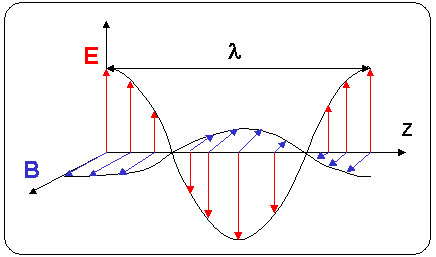
\includegraphics[scale=0.4]{OndeEM.png}
		\caption{Orientations vectorielles des champs}
	\end{figure}
\end{frame}








\end{document}